\documentclass[reqno,openany,12pt]{amsbook}
\usepackage{amsmath}
\usepackage[pdftex]{graphicx}

\usepackage{tikz}
\usetikzlibrary{mindmap,trees}
%  openany option dumps the blank pages between chapters when the next
%  chapter starts on odd page number; following command had similar
%  effect
%  \let\cleardoublepage\clearpage
%  NB need an abstract or get a blank page between title and contents


\renewcommand{\baselinestretch}{1.35}


%  ************  begin my definitions  *******************

% *** theorem etc. commands ***

\newtheorem{thm}{Theorem}%[section]
\newtheorem{lemma}[thm]{Lemma}
\newtheorem{cor}[thm]{Corollary}

\theoremstyle{definition}
\newtheorem{definition}[thm]{Definition}
\newtheorem*{ass}{Assumption S}

\theoremstyle{remark}
\newtheorem{remark}[thm]{Remark}

%\numberwithin{equation}{section}

\newenvironment{mylist}{\begin{enumerate}
\def\labelenumi{\theenumi}
\renewcommand{\theenumi}{(\roman{enumi})}
}{\end{enumerate}}

% *** greek commands ***

\newcommand\al{\alpha}
\newcommand\be{\beta}
\newcommand\ga{\gamma}
\newcommand\Ga{\Gamma}
\newcommand\de{\delta}
\newcommand\De{\Delta}
\newcommand\ep{\epsilon}
\newcommand\ka{\kappa}
\newcommand\la{\lambda}
\newcommand\La{\Lambda}
\newcommand\om{\omega}
\newcommand\Om{\Omega}
\newcommand\si{\sigma}
\newcommand\Si{\Sigma}
\renewcommand\th{\theta}
\newcommand\Th{\Theta}

% *** tilde/bar/bold commands ***


\newcommand\bg{\bar g}
\newcommand\bh{\bar h}
\newcommand\bu{\bar u}

\newcommand\bq{\boldsymbol{q}}
\newcommand\br{\boldsymbol{r}}
\newcommand\bv{\boldsymbol{v}}

% *** Bbb commands ***

\newcommand\Q{\mathbb{Q}}
\newcommand\R{\mathbb{R}}
\newcommand\Nf{\mathbb{N}}
\newcommand\Zf{\mathbb{Z}}

% *** script commands ***

\newcommand\I{{\mathcal I}}

\newcommand\B{{\mathcal B}}

% *** brackets commands ***

\newcommand\lan{\langle}
\newcommand\ran{\rangle}

% *** various maths commands ***

\newcommand\X{\times}
\newcommand{\tow}{\rightharpoonup}
\newcommand{\pa}{\partial}
\newcommand\rot{{\rm Rot}}


%  ************  end my definitions  *******************


\begin{document}


\title{Masters in Computer Vision\\Software Engineering Project\\2013-2014}
\author{Ozan\\Oksana\\Klemen\\Natalia\\
{\small
January 2014
}
}
\bigskip



%\begin{abstract}
%This project will investigate some aspects of rational approximation to
%real numbers.
%It is well known that any irrational number can be estimated arbitrarily
%close by rationals, i.e. for any $\ep>0$ and irrational $x \in \R$,
%there exists integers $p$,$q$ such that
%\begin{equation}  \label{abs_basic_app.eq}
%\left| {x-\frac{p}{q}} \right| < \ep
%\end{equation}
%This is known as Diophantine approximation, named after Diophantus of
%Alexandria.
%
%\end{abstract}


\maketitle


 \setcounter{page}{0}


\tableofcontents


\chapter{Introduction}

As a project at Software Engineering class we had to develop an application that to some extent mimics well known Google Earth. The main idea is to give an user who is unfamiliar with Le Creusot the tool that enables him to search for shortest path between two points on the map, enables him to create an itinerary containing different types of points of interest. We had to do all this in C++ and in Matlab.

\chapter{Project management}
In this chapter we want to present how our group organized and managed this project. As we all had a bit of software designing experiences, we knew how important a proper plan and research before the implementation is. Unfortunately, we were also aware that no matter how good the plan is, we will be forced to adjust it during the implementation, because of the things we did not take into account while planning or because some things turned out to be different to what we assumed. Because of that we decided to follow the iterative and incremental development model, which enabled us to adjust our plans after each of the implementation iterations. A schematic representation of the iterative and incremental development model can be seen on figure \ref{fig:Iterative_development_model_V2}. 
\begin{figure}[h]
\centering
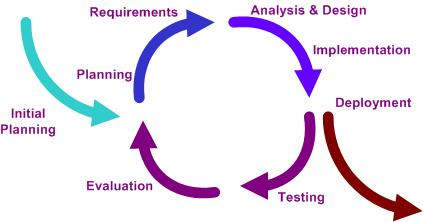
\includegraphics[height=4cm]{../photos/Iterative_development_model_V2}
\caption{An iterative development model}
\label{fig:Iterative_development_model_V2}
\end{figure}
\section{Basic building blocks}
To be able to fully manage the project at all times we decided to split the project into four main parts:
\begin{itemize}
\item User interface
\item Database
\item Map representation
\item Path algorithms
\end{itemize}
\begin{tikzpicture}
  \path[mindmap,concept color=gray,text=white]
    node[concept] {Project}
    [clockwise from=0]
    child[concept color=green!60!black] {
      node[concept] {User interface}
    }  
    child[concept color=blue] {
      node[concept] {Map representation}
    }
    child[concept color=red] { node[concept] {Path algorithms} }
    child[concept color=orange] { node[concept] {Database} };
\end{tikzpicture}
\subsection{UI - User Interface}\hspace*{\fill} \\
It is the part of the application that is responsible for user interaction with the application. Main goal is to make the interface as user-friendly as possible. In the beginning we made a rough sketch of how the interface should look (figure []), but we, as expected, changed it a little bit during the development. The UI is presented more in details in chapter [UI USER MAUNAL].
\subsection{Database}\hspace*{\fill} \\
Our database consists of two parts. The static part, having the information about the roads in Le Creusot (described in []) and the dynamic part with the information about the points of interest. From the beginning we were deciding between using XML based and relational database. During the consideration we took into account the following facts:
\begin{itemize}
\item Most of the data is static - information about the roads in Le Creusot will not change;
\item Dynamic data will change rarely - user will not often update information about the points of interest;
\item Relatively small amount of data - Le Creusot is a small city, so there is not a lot of information about the roads. This gives us the opportunity to read all the information to memory at the beginning, reducing the latency caused by queries to the database;
\item Easiness of install and mobility -  using relational database, requires installation of different software (sql server, connectors, etc.) on the clients computer, which we wanted to avoid. 
\end{itemize}  
Because of all these reasons we decided to use XML based database. We have the information about the roads in one osm file, while the information about the points of interest is in xml file. We will describe both of them more  in detail in later chapters.
\subsection{Map representation}\hspace*{\fill} \\
TODO
\subsection{Path algorithms}\hspace*{\fill} \\
This part consists of all calculations about paths, distances, travelling times and optimizations of the paths. Our main goal is to make the algorithms work as quickly as possible, taking into account all the restrictions road networks has (oneway streets, footways etc.). We also want to make the algorithms as reusable as possible, to reduce the redundancy in development and minimize the possibilities of errors.
\section{Softwares used for project management}
Github, skype etc.
\section{Meetings}
some bullshit about that

\chapter{Initial planning}
As already mentioned in the previous chapter, we decided to use the iterative and incremental development model. Before starting the iterations we spend quite a lot of time on the initial planning, with special attention to user and general project requirements analysis. From the project's instructions we were able to identify the following major user requirements and construct use case diagram:
\begin{itemize}
\item user should be able to enter start and end point either by:
\begin{itemize}
\item mouse click
\item specifying latitude and longitude
\item selecting a point of interest
\end{itemize}
\item find shortest path from point A to point B (by foot or by car)
\item find all points of interest in a certain radius from point A (by foot or by car)
\item construct an itinerary from point A to point B with points of interest in between (with max distance limit)
\item view, edit and add points of interest (POI)
\end{itemize}
For better 
\section{Shortest path A -> B}
\section{title}
!!!ADD image of the use case diagram
\chapter{Plan of implementation}
After having the user requirements, we decided to make the global plan of implementation. Here we had to take into account, that we have to develop the application in C++ and Matlab. As show in the figure[] we have already splited  the project into four main parts. Because the user interface and map representations require completely different approaches in C++ and Matlab, we decided to split them into two parallel projects, one almost independent from another. On the other hand, we decided to use the same algorithms for both projects. The main reason was to minimize the redundancies in the research and development stage and minimize the possibility of errors. This way we could have the same algorithms for both, differing only in pure implementation details. \\
\\ Each of was delegated to oversee one of the parts (as shown in figure []). We have to emphasis that this does not mean he/she developed that part by him/herself, not even that he is solely responsible for it. No matter the delegation, we all worked on all parts of the project, either in research, design or implementation stage.



\chapter{Path algorithms}
\section{Street data}
What did we use...open street map...shot introduction into nodes, relations etc.
\section{DB class structure}
\section{Algorithms - shortest path}
\subsection{A*}
\section{Radius search}
\section{Bicycle search}
\chapter{GUI}
\section{C++}
\subsection{UI}
\subsection{OpenGL}
\section{Matlab}
\subsection{UI}
\subsection{library for maps}
\chapter{c++ vs matlab}




\begin{thebibliography}{99}

\bibitem{Bovey}
J. D. Bovey, M. M. Dodson,
The Hausdorff dimension of systems of linear forms
{\em Acta Arithmetica}
(1986) 337-358.

\bibitem{Cassels}
J. W. S. Cassels,
{\em An Introduction to Diophantine Approximation},
Cambridge University Press, 1965.



\end{thebibliography}


\end{document}
